\clearpage

\section{IQ Modulator}
\begin{refsection}
\begin{tcolorbox}	
	\begin{tabular}{p{2.75cm} p{0.2cm} p{10.5cm}} 	
		\textbf{Header File}   &:& iq\_modulator.h \\
		\textbf{Source File}   &:& iq\_modulator.cpp \\
		\textbf{Source File}   &:& 20180130 \\
		\textbf{Source File}   &:& 20180828 (Romil Patel)\\	
	\end{tabular}
\end{tcolorbox}
\subsection*{Version 20180130}
This blocks accepts one inupt signal continuous in both time and amplitude and it can produce either one or two output signals. It generates an optical signal and it can also generate a binary signal.
\subsection*{Input Parameters}
\begin{table}[h]
	\centering
	\begin{tabular}{|c|c|c|c|cccc}
		\cline{1-4}
		\textbf{Parameter} & \textbf{Type} & \textbf{Values} &   \textbf{Default}& \\ \cline{1-4}
		outputOpticalPower & double & any & $1e-3$ \\ \cline{1-4}
		outputOpticalWavelength & double & any & $1550e-9$ \\ \cline{1-4}
		outputOpticalFrequency & double & any & speed\_of\_light/outputOpticalWavelength \\ \cline{1-4}
	\end{tabular}
	\caption{Binary source input parameters}
	\label{table:iqmod_in_par}
\end{table}
\subsection*{Methods}
IqModulator(vector$<$Signal *$>$ \&InputSig, vector$<$Signal *$>$ \&OutputSig) :Block(InputSig, OutputSig)\{\};
\bigbreak
void initialize(void);
\bigbreak
bool runBlock(void);
\bigbreak
void setOutputOpticalPower(double outOpticalPower)
\bigbreak
void setOutputOpticalPower$\_$dBm(double outOpticalPower$\_$dBm)
\bigbreak
void setOutputOpticalWavelength(double outOpticalWavelength)
\bigbreak
void setOutputOpticalFrequency(double outOpticalFrequency)
\subsection*{Functional Description}
This block takes the two parts of the signal: in phase and in amplitude and it combines them to produce a complex signal that contains information about the amplitude and the phase.
This complex signal is multiplied by $\frac{1}{2}\sqrt{\textit{outputOpticalPower}}$ in order to reintroduce the information about the energy (or power) of the signal. This signal corresponds to an optical signal and it can be a scalar or have two polarizations along perpendicular axis. It is the signal that is transmited to the receptor.
The binary signal is sent to the Bit Error Rate (BER) meaurement block.
\subsection*{Input Signals}
\subparagraph*{Number}: 2
\subparagraph*{Type}: Sequence of impulses modulated by the filter (ContinuousTimeContiousAmplitude))
\subsection*{Output Signals}
\subparagraph*{Number}: 1 or 2
\subparagraph*{Type}: Complex signal (optical) (ContinuousTimeContinuousAmplitude) and binary signal (DiscreteTimeDiscreteAmplitude)
\subsection*{Example}
\begin{figure}[h]
	\centering
	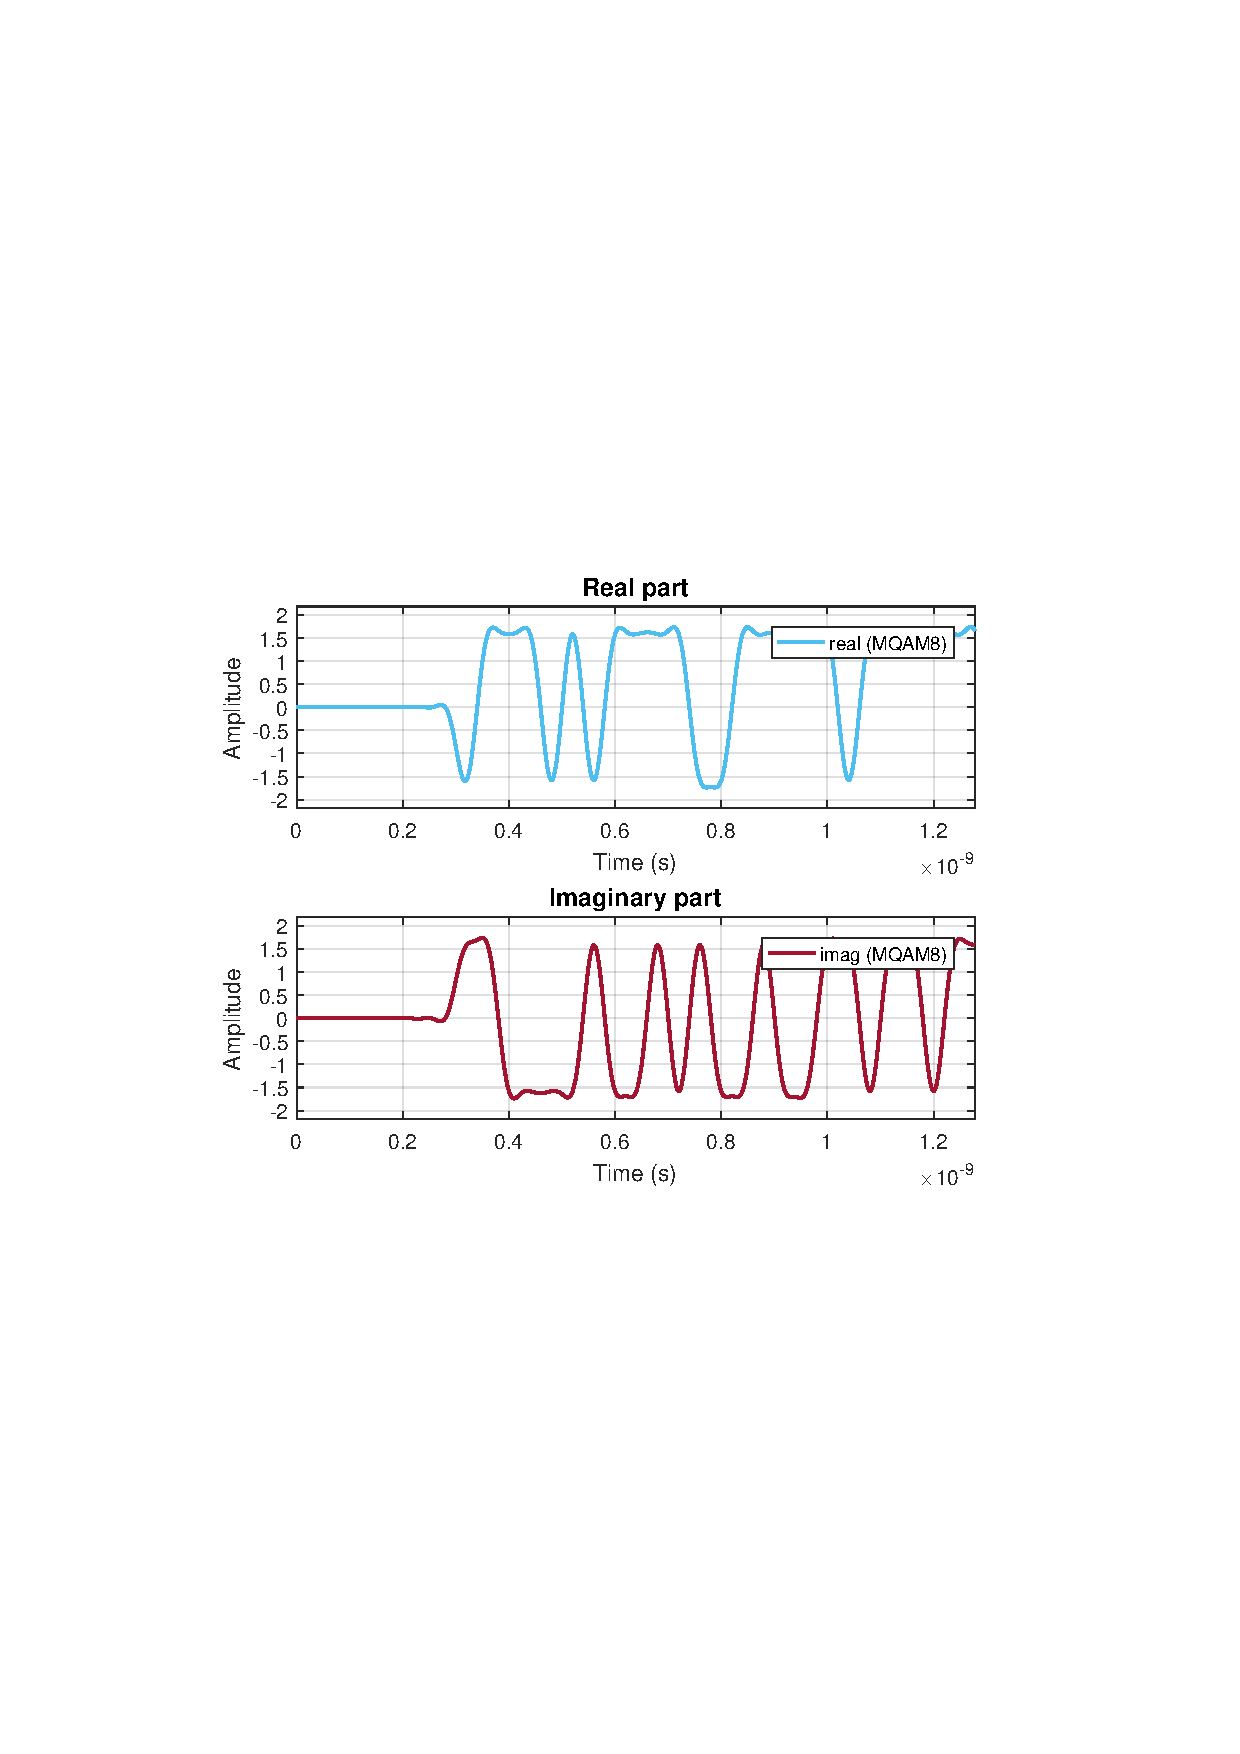
\includegraphics[width=1.0\textwidth, height=7cm]{./lib/iq_modulator/figures/MQAM_iq_modulator_output.pdf}
	\label{MQAM8_DeterministicAppendZeros}\caption{Example of a signal generated by this block for the initial binary signal 0100...}
\end{figure}
%%%%%%%%%%%%%%%%%%%%%%%%%%%%%%%%%%%%%%%%%%%%%%%%%%%%%%%%%%%%%%%%%%%%%%%%%%%%%%%%%%%%%%%%%%%%%%%%%%
\subsection*{Version 20180828}
\subsection*{Input Parameters:}
---NA---

\subsection*{Input Signals:}
\textbf{Number}: 1, 2,3\\
\textbf{Type}: RealValue
\subsection*{Output Signals:}
\textbf{Number}: 4\\
\textbf{Type}: RealValue

\subsection*{Functional Description}
This blocks has three inputs and one output. Port number 1 and 2 accept the real and imaginary data respectively and port 3 accepts the local oscillator as an input to the IQ modulator. This model serves as an ideal IQ modulator without noise and introduction of nonlinearity.
\begin{figure}[h]
	\centering
	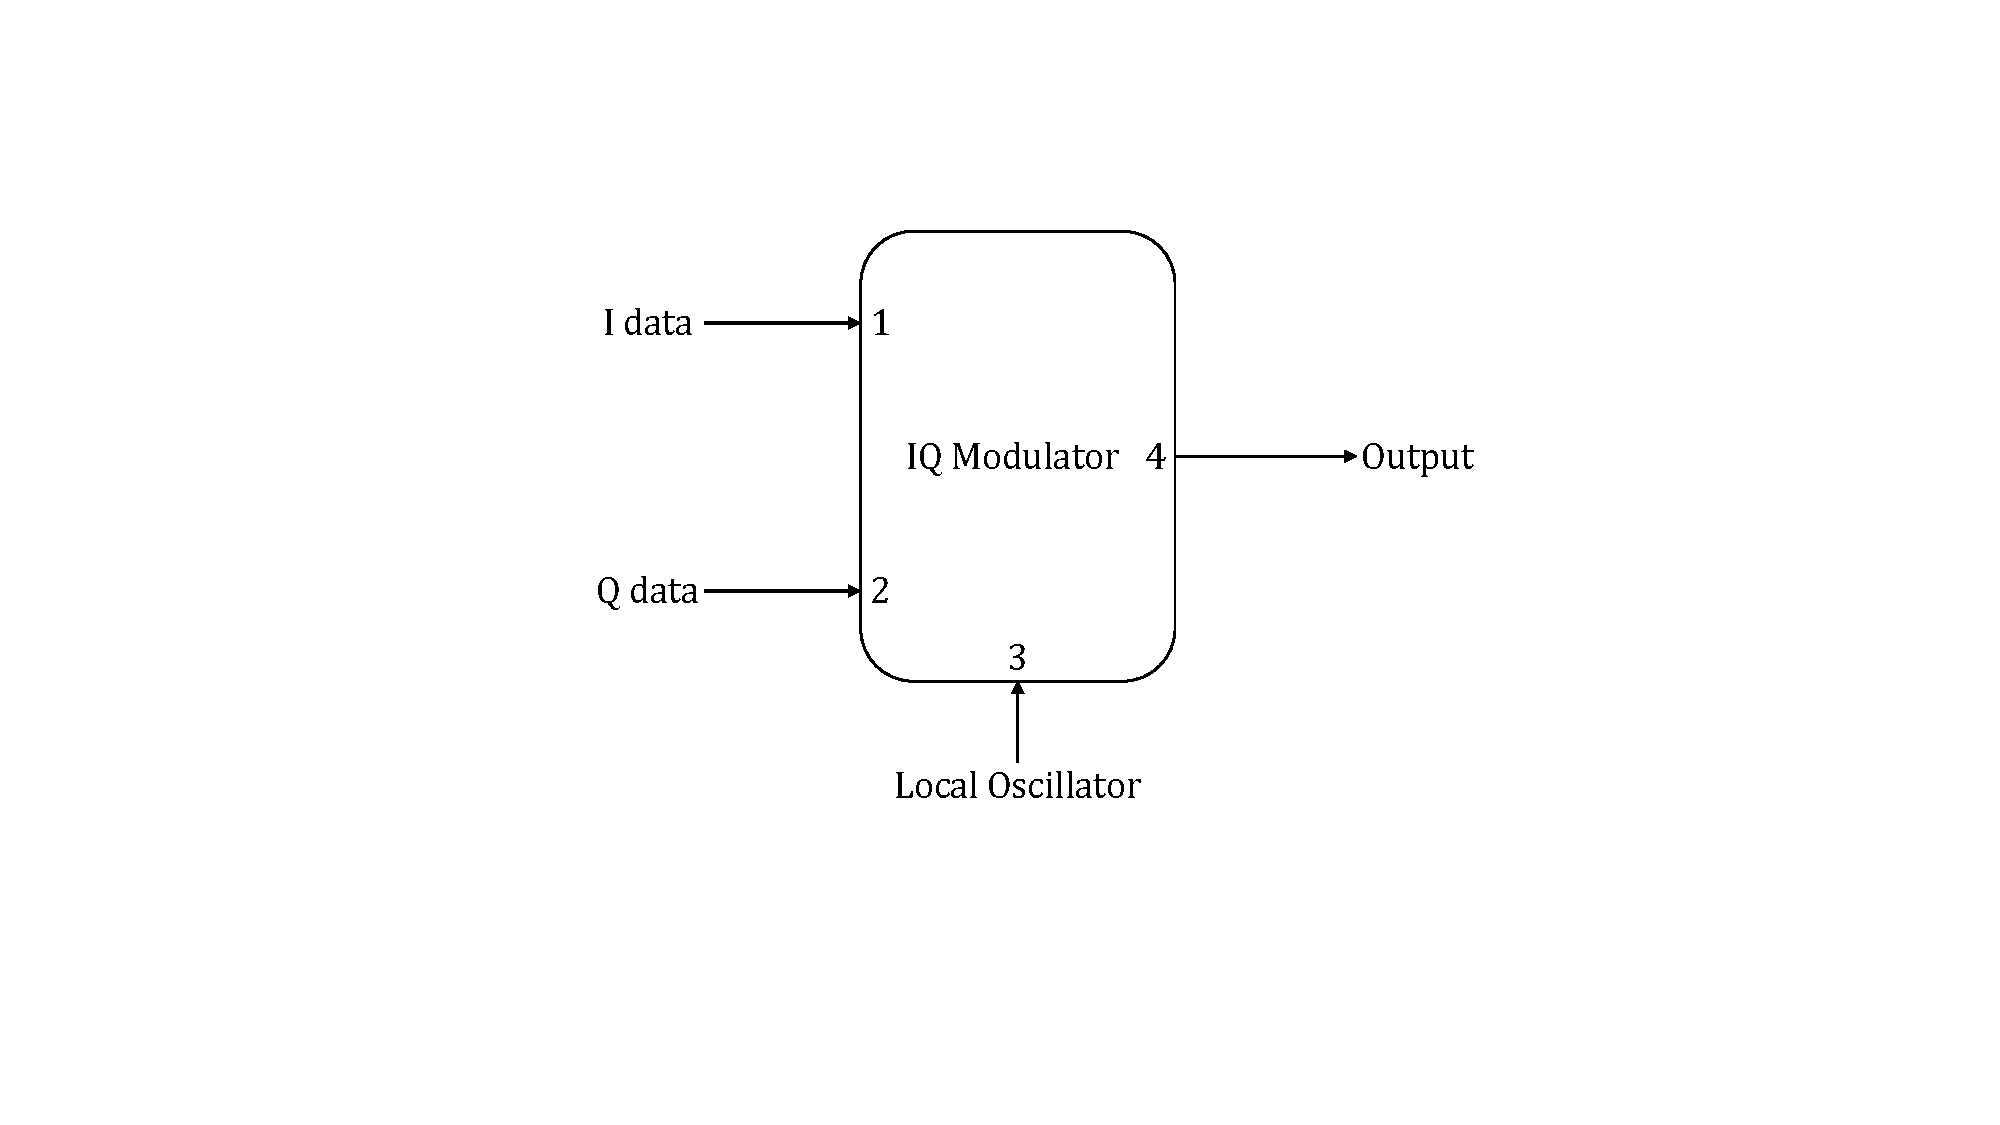
\includegraphics[width=0.75\textwidth, height=6cm]{./lib/iq_modulator/figures/IQ_modulator_block.pdf}
	\label{IQ_modulator_block}\caption{IQ Modulator block}
\end{figure}

\subsection*{IQ MZM Description}
The detailed expatiation of the MZM starts with the phase modulator (see Figure \ref{Phase_Modulator}). The transfer function of the phase modulator can be given as,
\begin{figure}[h]
	\centering
	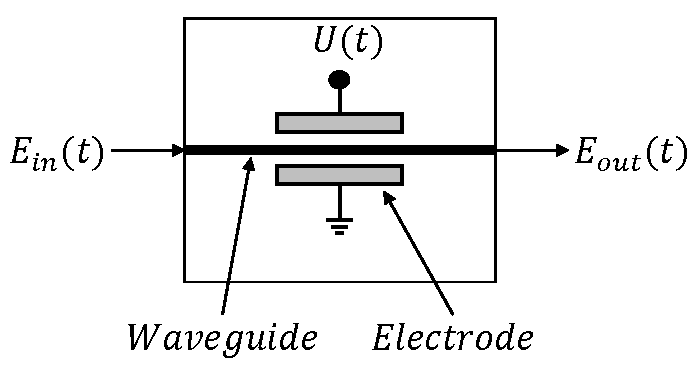
\includegraphics[width=0.6\textwidth, height=5cm]{./lib/iq_modulator/figures/PM.pdf}
	\label{Phase_Modulator}\caption{Phase Modulator}
\end{figure}
\begin{equation*}
E_{out}(t)=E_{in}(t)\cdot e^{j\phi_{PM}(t)} = E_{in}(t)\cdot e^{j\frac{u(t)}{V_{\pi}}\pi}
\label{PM_TF}
\end{equation*}
Two phase modulators can be placed in parallel using an interferometric structure as shown in Figure \ref{MZM}. The incoming light is split into two branches, different phase shifts applies to each path, and then recombined.
The output is a result of interference, ranging from constructive (the phase of the light in each branch is the same) to destructive (the phase in each branch differs by $\pi$). 
\begin{figure}[h]
	\centering
	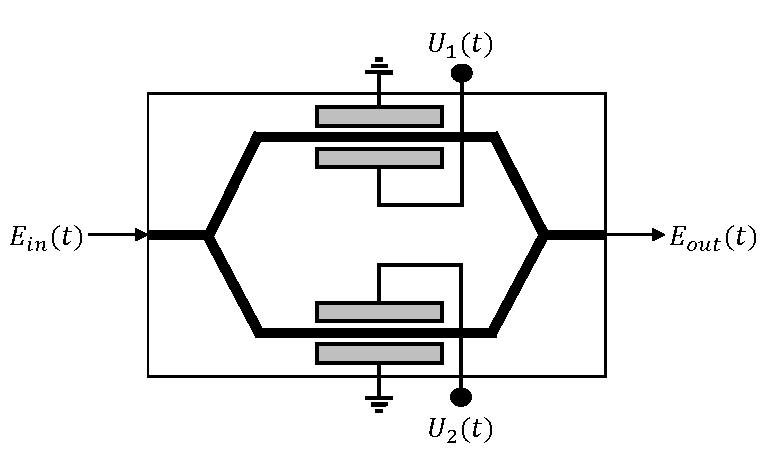
\includegraphics[width=0.6\textwidth, height=5cm]{./lib/iq_modulator/figures/MZM.pdf}
	\label{MZM}\caption{Mach-Zehnder Modulator}
\end{figure}
The transfer function of the structure can be given as,
\begin{equation}
\dfrac{E_{out}(t)}{E_{in}(t)} = \frac{1}{2}\cdot(e^{j\phi_{1}(t)}+e^{j\phi_{2}(t)})
\label{MZM_TF}
\end{equation}
Where, $\phi_{1}(t)=\frac{u_{1}(t)}{V_{\pi_{1}}} \pi$ and  $\phi_{2}(t)=\frac{u_{2}(t)}{V_{\pi_{2}}} \pi$. if the inputs are set to $u_{1}=u_{2}$ (push-push operation) then it provides the pure phase modulation at the output. Alternatively, if the inputs are set to $u_{1}=-u_{2}$ (push-pull operation) then it provides pure amplitude modulation at the output.\\
The structure of the IQ MZM can be represented  shown in Figure \ref{IQ_Mach-Zehnder_Modulator} where the incoming source light spitted into two portions. The first portion will drive the MZM of the I-channel and other portion will drive MZM Q-channel data. In the Q-channel, before feeding it to the MZM, it passed though the phase modulator to provide a $\pi /2$ phase shift to the carrier. The output of the MZM combined to form the electrical field $E_{out}(t)$ \cite{NPTEL}. 
\begin{figure}[h]
	\centering
	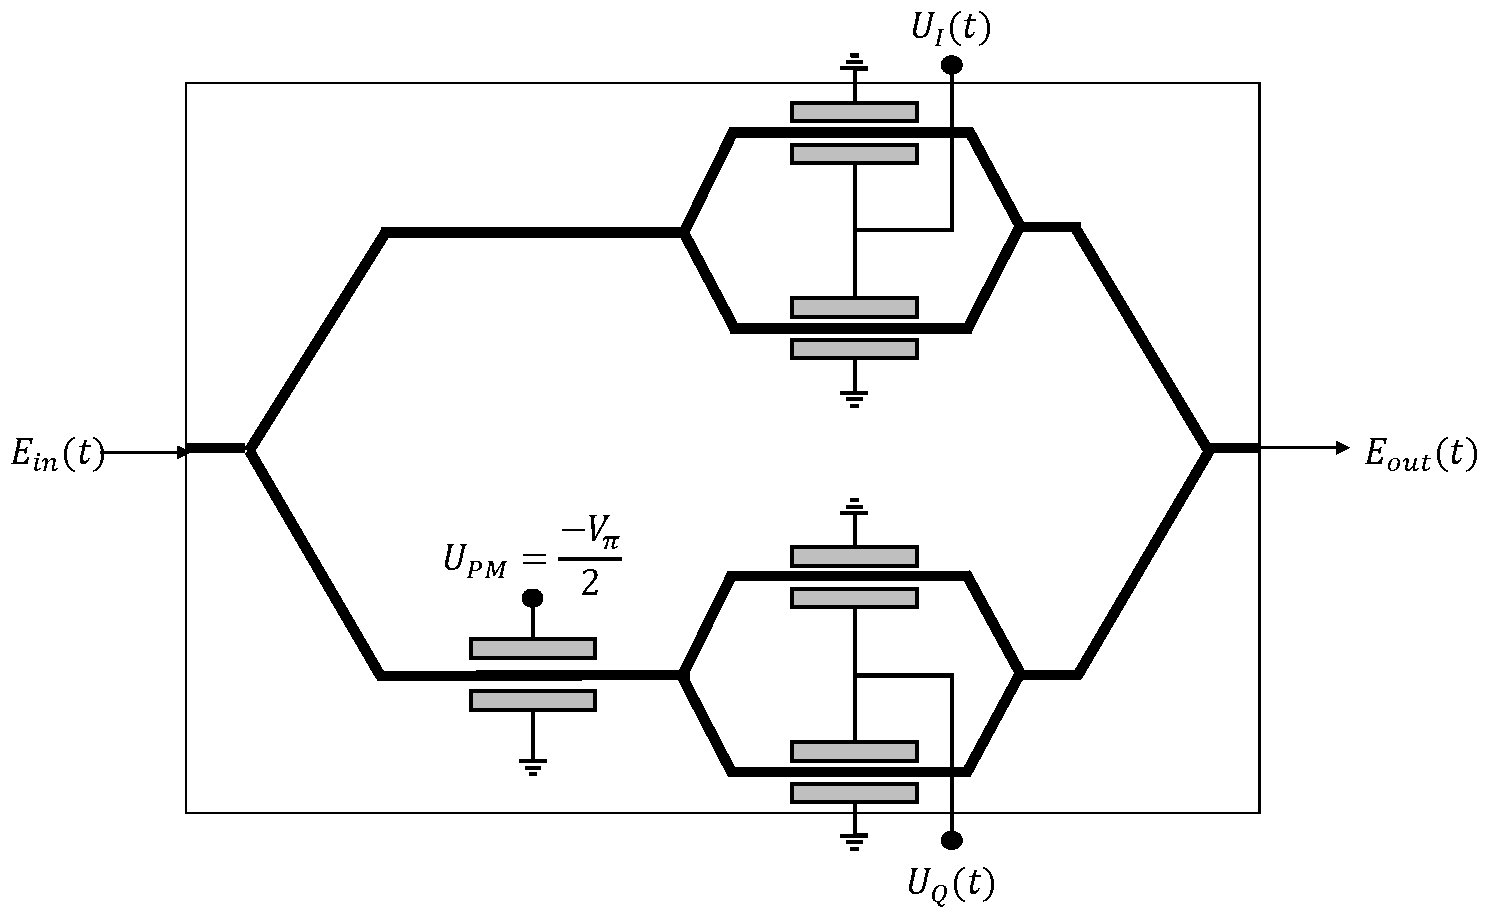
\includegraphics[width=0.9\textwidth, height=8cm]{./lib/iq_modulator/figures/IQ_MZM.pdf}
	\label{IQ_Mach-Zehnder_Modulator}\caption{IQ Mach-Zehnder Modulator}
\end{figure}
The transfer function of the IQ MZM can be written as,
\begin{equation}
E_{out}(t)=\frac{1}{2}{E_{in}(t)} \bigg[cos\big(\dfrac{\pi U_{I}(t)}{2 V_{\pi}}\big) + j \cdot cos\bigg(\dfrac{\pi U_{Q}(t)}{2 V_{\pi}}\bigg) \bigg] 
\label{IQ_MZM_TF}\
\end{equation}
The black  box model of the IQ MZM in the simulator can be depicted as,
 \begin{figure}[h]
 	\centering
 	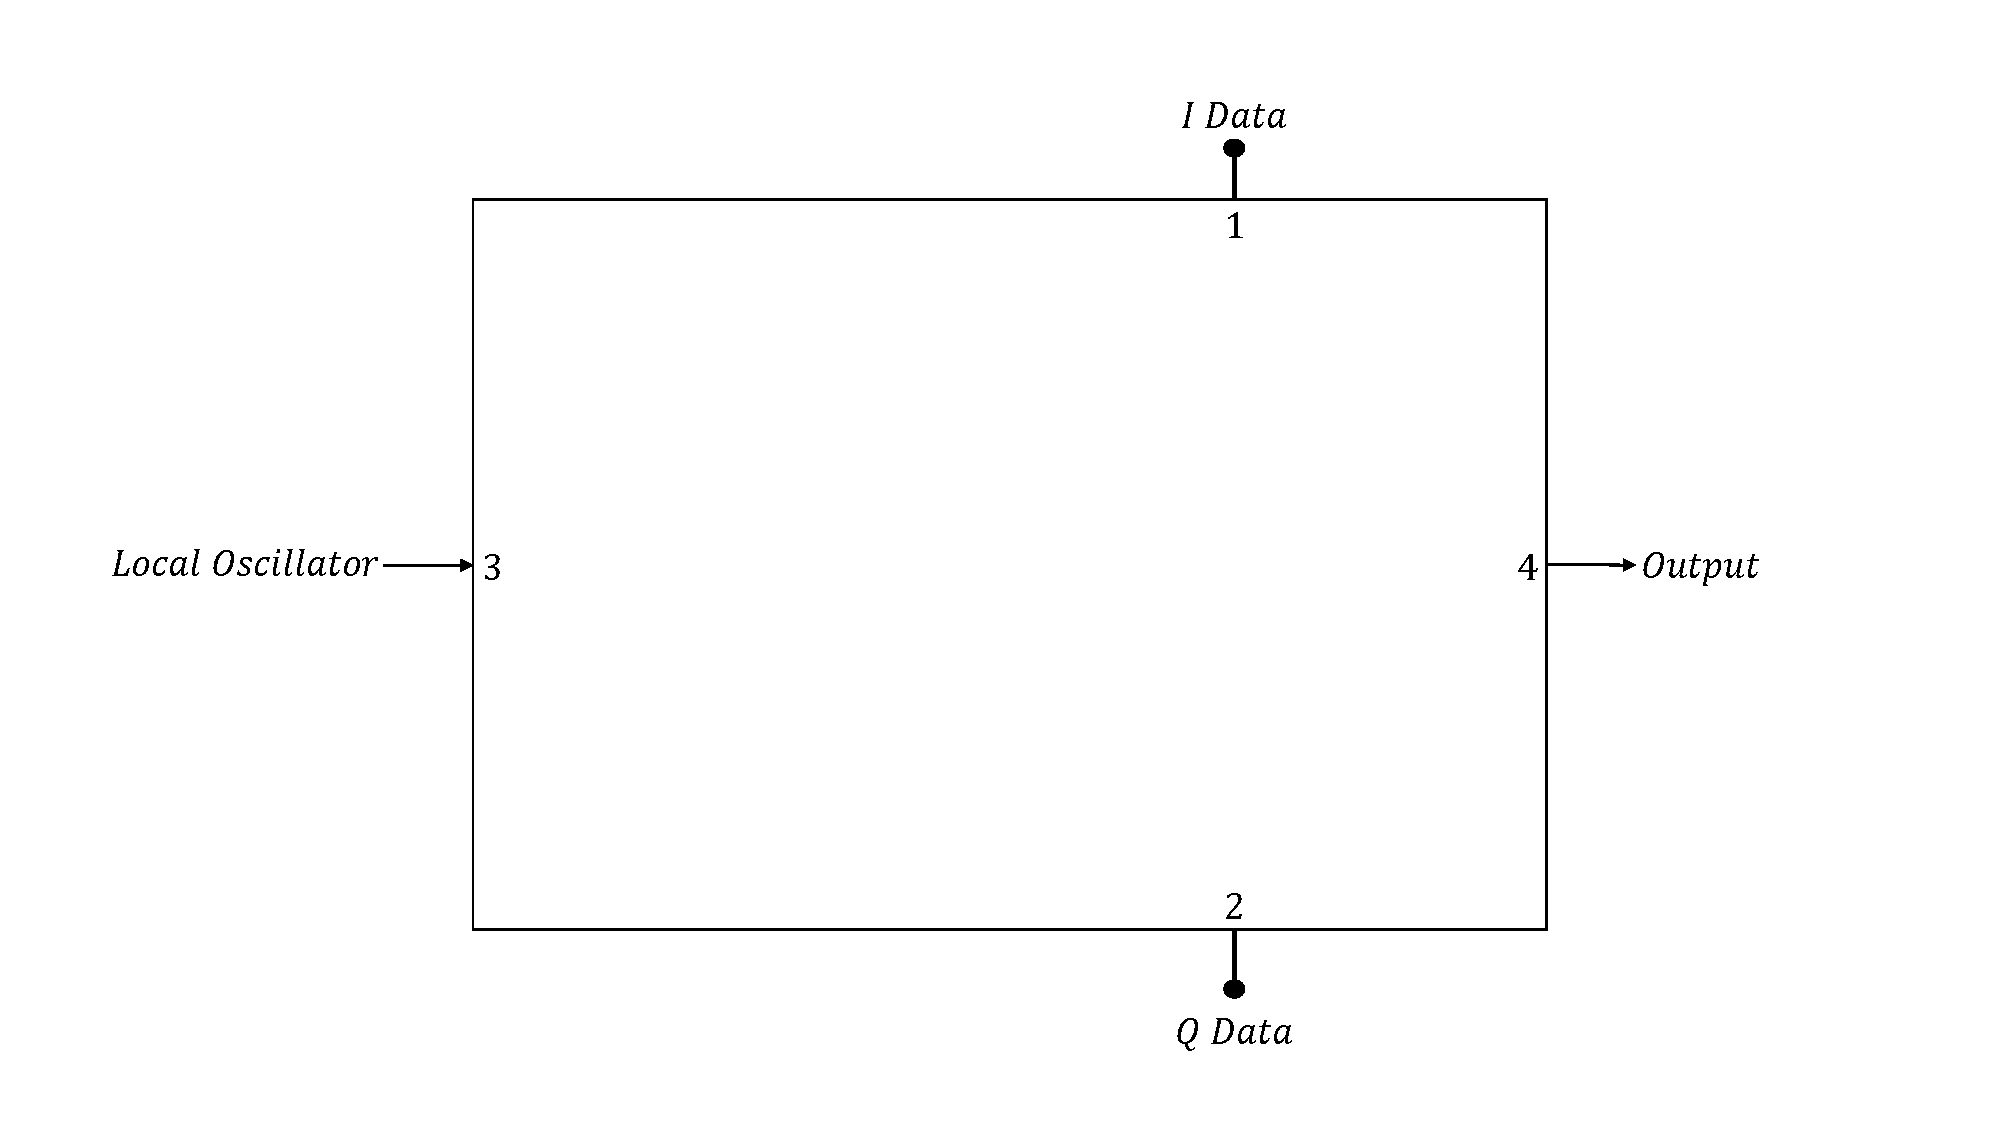
\includegraphics[width=0.9\textwidth, height=8cm]{./lib/iq_modulator/figures/Black_Box.pdf}
 	\label{Black_Box}\caption{Simulation model of the IQ Mach-Zehnder Modulator}
 \end{figure}

% Bibliography
\clearpage
\printbibliography[heading=subbibliography]
\end{refsection}
\addcontentsline{toc}{subsection}{Bibliography}
\cleardoublepage
